\subsection{Funktionsnachweis kritischer Funktionen}
\label{funktionsnachweis}
\textit{(ygu)} Dieses Unterkapitel befasst sich mit dem praktischen Nachweis von kritischen Teilfunktionen. Kritische Teilfunktionen sind Funktionen, welche bei einem Ausfall, einen Ausfall des Gesamtsystems zur Folge hat. Daher wird die technische Machbarkeit dieser Teillösungen zusätzlich überprüft. Einfach aufgebaute aber funktionell ähnliche Versuche werden realisert. An diesen Aufbauten wird dann der praktische Nachweis erbracht, ob die techische Umsetzbarkeit realistisch erscheint. Diese Beurteilung wird für Bewertung der ausgearbeiteten Lösungskonzepte miteinbegezogen.
\newline
Bei Betrachtung der Funktionsanalysen (Abbildungen \ref{fig:FunktPflicht} und \ref{fig:FunktWunsch}) ist erkennbar, dass beide Varianten (Pflicht sowie Wunsch) eine Serieschaltung darstellen.  Bei der Umsetzung einer Maschine mit einfacher Redundanz ergibt dies implizit, dass jede Funktion als kritisch eingestuft wird. Aus zeitlichen Gründen kann ein umfassenden Nachweis von allen Teillösungskonzepten nicht abschliessend durchgeführt werden. Für den Nachweis ist eine pragmatische Auswahl notwendig. Es werden daher nur Funktionen mit erhöhtem Ausfallrisiko und einer vielversprechenden Funktionserfüllung überprüft.

\subsubsection{NemaCaps vereinzeln und fördern}
Die Automatisationsbranche setzt sich vertieft mit der Förderung und Vereinzelung von Gütern auseinander. Die automatisierte Sortierung sowie Transport eines Gutes sind grundlegende Bedingungen, sodass ein Produkt überhaupt in der automatisierten Serienfertigung herstellbar wird. Da solche Lösungen vielfach beide Funktionen miteinander vereinen, werden diese gemeinsam in einem Unterkapitel untersucht.
\newline
\newline
\textbf{Vibrationswendelförderer}
\newline
Der Vibrationswendelförderer ist ein Bestandteil von Konzept Grün. Die detaillierte Funktionsweise des Vibrationswendelförderers wurde bereits im Kapitel \ref{KonzeptGreen} erläutert.
\newline
Aus vergangenen Studentenarbeiten besitzt die HSLU T\&A solch ein Wendelförderer. Dimensioniert ist dieser für die Vereinzelung von gezuckerten Mandeln. Auch wenn dadurch die Vereinzelung nur bedingt funktionsfähig ist, eignet sich dieses Gerät zur ersten Überprüfung mit NemaCaps. 

Praktische Tests mit NemaCaps konnten am 15.3.2017 am Wendelförderer durchgeführt werden. NemaCaps wurden ins Haufwerk (Punkt 1 in Abbildung \ref{fig:wendelfoerderer}) eingefüllt und der Wendelförderer gestartet. Durch die Vibration sammelten sich die NemaCaps im Wendel (2) und begannen zu wandern. Die Förderung klappte einwandfrei, wobei die rasche Transportgeschwindigkeit positiv überraschte. 
\begin{figure}[H]
	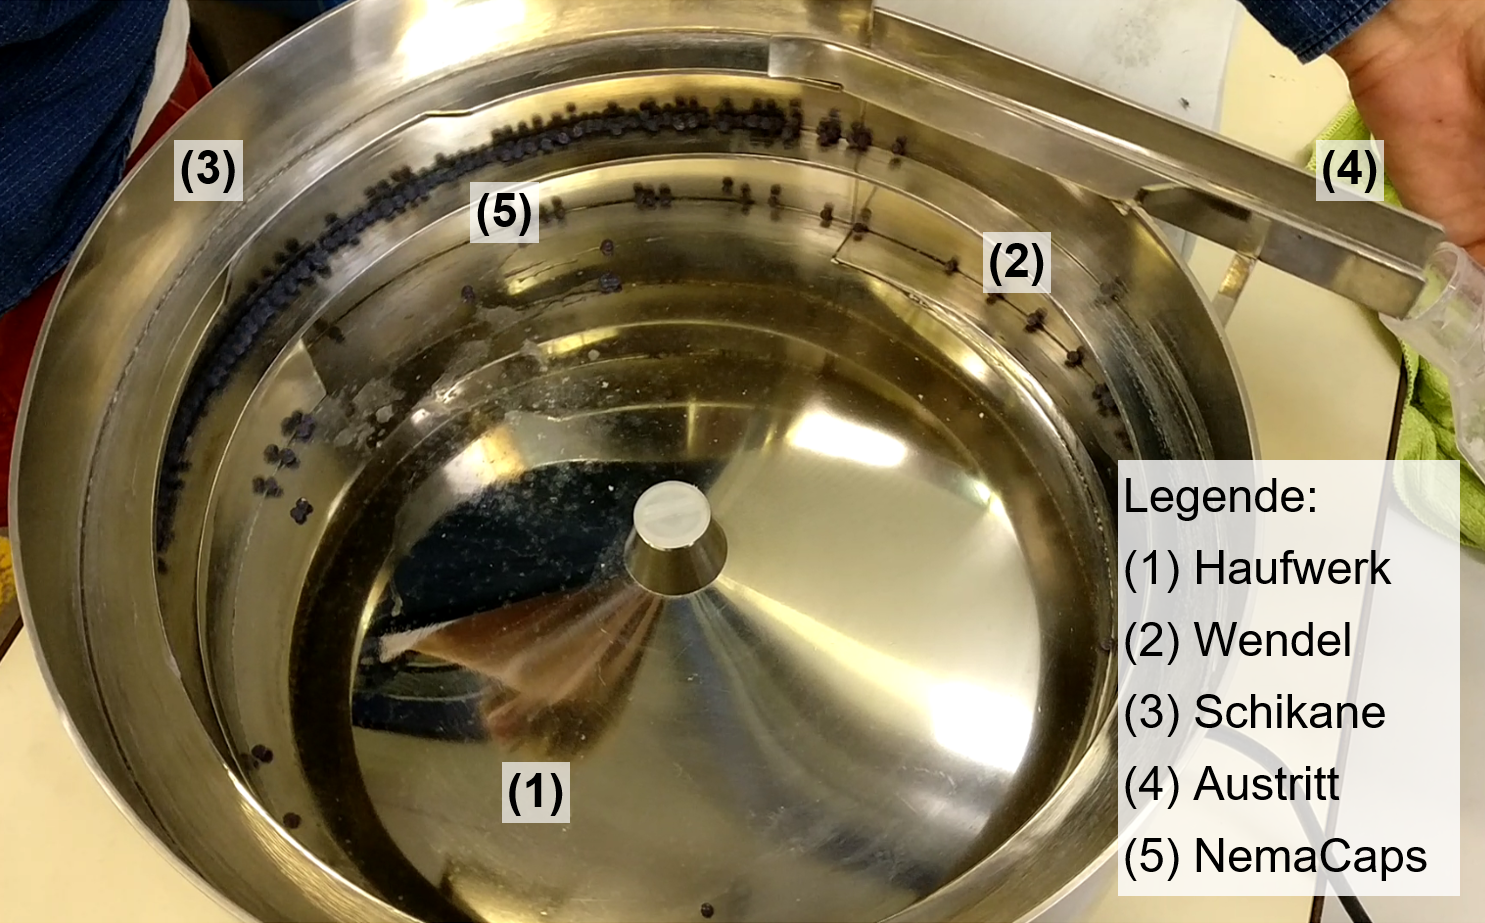
\includegraphics[width=1\textwidth]{Illustrationen/5-Konzept/wendelfoerderer.PNG}
	\caption{Praktische Tests am Wendelförderer der Hochschule}
	\label{fig:wendelfoerderer}
\end{figure}
\textbf{Erkenntnisse}
\newline
Folgende Erkenntnisse lieferten die Versuche:
\begin{itemize}
	\item Eine Förderung von NemaCaps mit einem Wendelförderer ist möglich. Die NemaCaps eignen sich als Fördergut und werden mit einer hohen Zuverlässigkeit gefördert.
	
	\item Die Schikane erfüllt ihre Funktion nicht. Dies ist allein auf die Tatsache zurückzuführen, dass der verwendete  Wendelförderer für gezuckerte Mandeln dimensioniert wurde. Eine Anpassung der Schikanen auf NemaCaps ist technisch machbar.
	
	\item Die Umsetzung der Funktionen 'NemaCaps vereinzeln' und 'NemaCaps fördern' mit einem Wendelförderer ist aus rein technischer Sicht realisierbar.
\end{itemize} 
\newpage
\textbf{Vereinzelung durch Lochmaske}
\newline
Die Vereinzelung durch eine rotierende Lochmaske ist Teil von Konzept Blau. Der praktische Funktionsnachweis wird anhand eines einfachen Funktionsmusters erbracht. Eine manuell drehbare Lochmaske wird dabei auf einer schief gelagerten Grundplatte montiert (siehe Abbildung \ref{fig:funktmuster_vereinzelung}). Auf der Grundplatte ist eine gewölbte Wand verklebt, die zur Lagerung der NemaCaps dient. Das Design des Funktionsnachweises ist jenem der Firma Kofatec GmbH angelehnt. Die Lochmaske wird für einen ersten Funktionsnachweis von Hand betrieben.
\begin{figure}[H]
	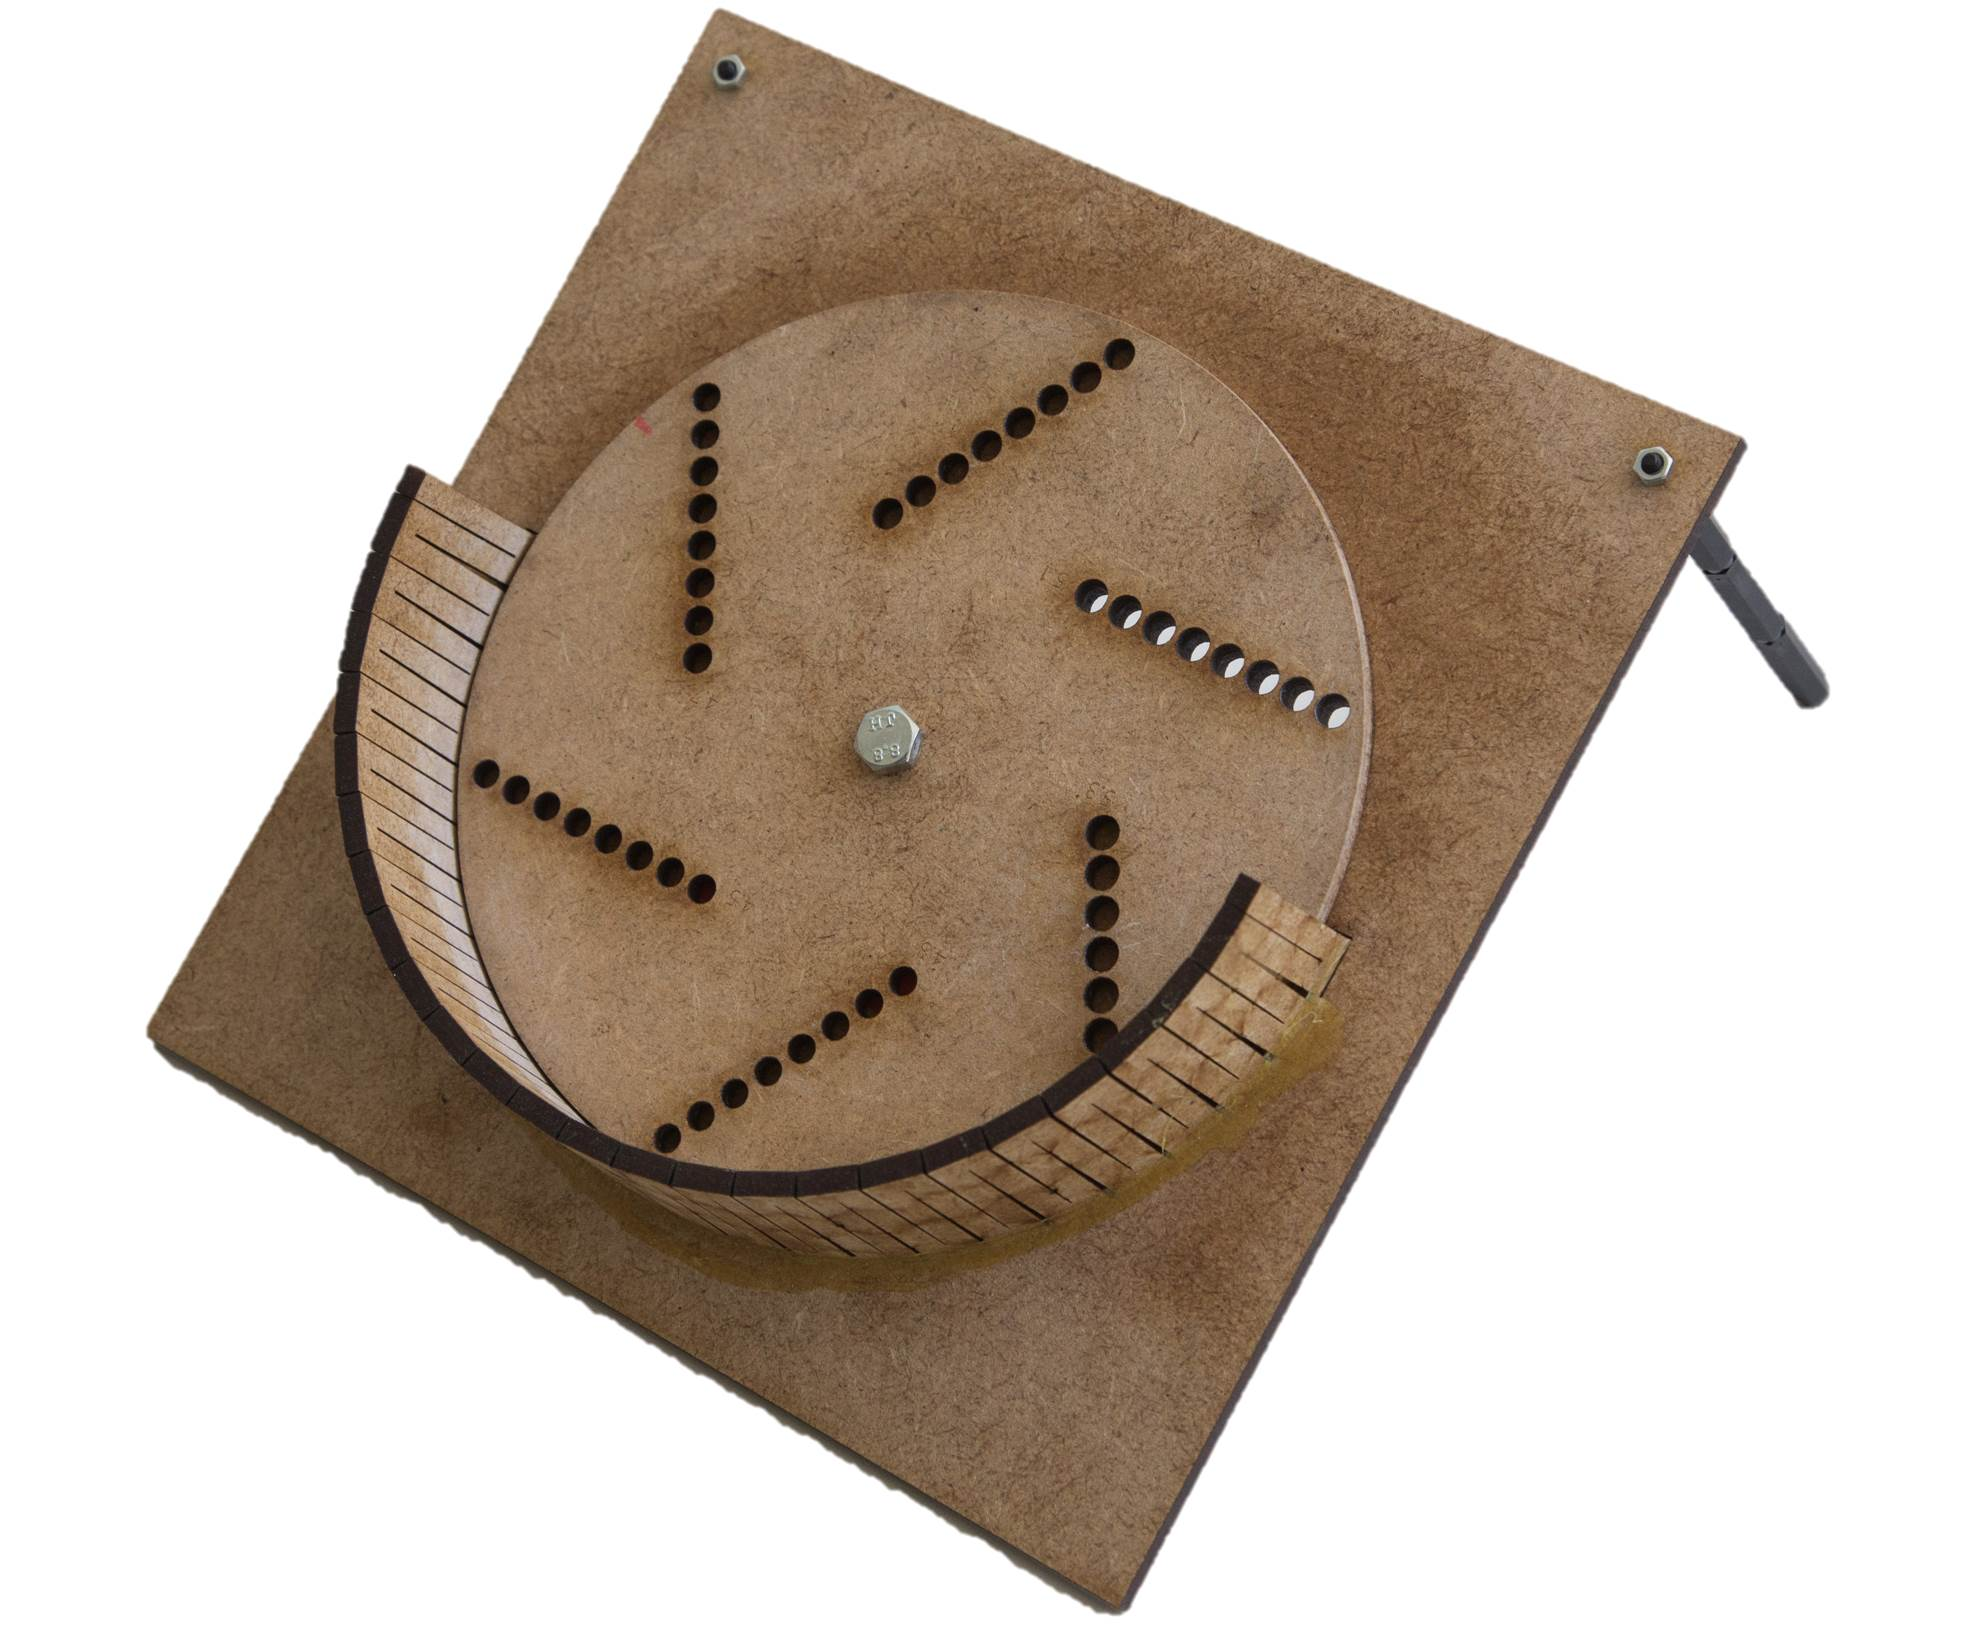
\includegraphics[width=1\textwidth]{Illustrationen/5-Konzept/funktmuster_vereinzelung_1.jpg}
	\caption{Teilfunktionsmuster zur Vereinzelung der NemaCaps}
	\label{fig:funktmuster_vereinzelung}
\end{figure}
Am 21.3.2017 wurde am umgesetzten Funktionsmuster der Funktionsnachweis durchgeführt. Durch zielgerichtetes Ausprobieren von verschiedenen Durchmesser der Löcher wurde die Lochmaske für die NemaCaps ausgelegt. Anschliessend wurde mittels manuellem Rotieren die Vereinzelung überprüft.
\begin{figure}[H]
	\includegraphics[width=1\textwidth]{Illustrationen/5-Konzept/funktion_vereinzelung.jpg}
	\caption{Funktionsnachweis der Vereinzelung}
	\label{fig:funktion_vereinzelung}
\end{figure}
Folgende Erkenntnisse lieferten die Versuche:
\begin{itemize}
	\item Die Lochmaske nimmt zuverlässig NemaCaps auf (Siehe Punkt 2 und Detail A in Abb. \ref{fig:funktion_vereinzelung}). Auch ein Transport zur Auslösung verläuft problemlos.
	
	\item Die Abstreifung von NemaCaps funktioniert. Kritisch ist dabei jedoch die Wahl des Abstreifers. Verwendet man scharfkantige Gegenstände kann es passieren, dass NemaCaps beschädigt werden. Weiter wurde erkannt, dass NemaCaps heikel auf Scherkräfte reagieren.
		
	\item Die Zuverlässigkeit der Auslösung am Punkt 3 in Abb. \ref{fig:funktion_vereinzelung} ist durchschnittlich. Dies wird damit erklärt, dass nicht frische NemaCaps verwendet wurden. Dadurch hat sich das hygroskope Pulver in Wasser gewandelt und so die Adhäsion der NemaCaps erhöht. Dadurch blieben geschätzte 50 Prozent der NemaCaps an der Lochmaske hängen. Auch ist ein holzfaserbasiertes Material (wie MDF) für die Lochmaske ungeeignet. Die rauhe Oberfläche der Bohrung bietet so mehr Haftung.
	
	\item Durch leichtes Antippen der Grundplatte oder einem Luftstoss konnten alle NemaCaps ausgelöst werden. Dies zeigt, dass durch Abhilfemassnahmen durchaus eine höhere Zuverlässigkeit erreicht wird.
	
	\item Die Umsetzung von diesem Lösungsansatz ist nur realistisch, wenn klare Abhilfemassnahmen und Verbesserungen der Lochmaske zur Steigerung der Zuverlässigkeit definiert werden. 
\end{itemize} 


\subsubsection{NemaCaps setzen}
\label{nemacaps_setzen}
Der Lösungsansatz der Teilfunktion 'NemaCaps setzen' basiert auf der Idee, in einem ersten Schritt ein Loch auszuheben oder Erde zu verdrängen und anschliessend ein NemaCap in die Vertiefung fallen zu lassen. Ein ähnlicher Ansatz verfolgt die Idee, mit einer spitzen Zange Erde zu verdrängen, die Zange im Erdreich zu öffnen und dort ein NemaCap zu platzieren. Schematisch dargestellt sind beide Ansätze in Abbildung \ref{fig:skizze_setzversuch}.
\newline
Um die Umsetzbarkeit dieser Ideen zu überprüfen, werden zwei Versuche durchgeführt:
\begin{itemize}
	\item \textbf{A) Ermittlung der Verdrängkraft:} Mit einer konventionellen Setzhilfe aus dem Gartenbau werden praktische Tests durchgeführt. Ein Topf wird mit dem vorgegebenen Gartenhumus von Ricoter befüllt und leicht angepresst. Anschliessend wird die maximale Einsetztiefe an der Setzhilfe markiert und schrittweise mit Gewicht (Masse m in Abbildung \ref{fig:skizze_setzversuch}) beschwert. Sobald die Markierung den Gartenhumus berührt, wird die Setzhilfe inklusive Masse m gewogen und durch die Multiplikation mit der Erdbeschleunigung die benötigte Verdrängungskraft ermittelt.
		
	\item \textbf{B) NemaCap mittels Zange setzen:} Der identische Versuch wird mit der genannten Zange durchgeführt, wobei die geschlossene Zange ein NemaCap gegeben wird. Bei Erreichung der Setztiefe wird die Zange geöffnet und das NemaCap platziert (siehe Abbildung \ref{fig:skizze_setzversuch}).
\end{itemize} 

\begin{figure}[H]
	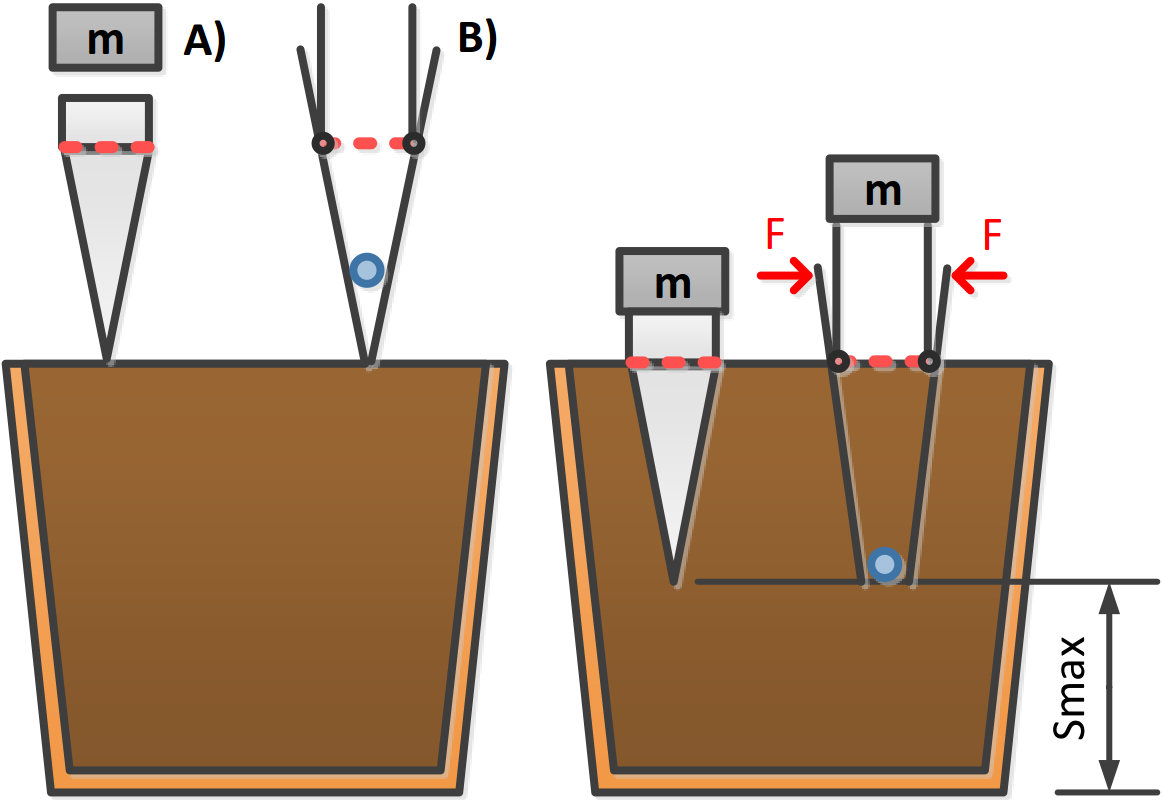
\includegraphics[width=1\textwidth]{Illustrationen/5-Konzept/skizze_stechversuch.PNG}
	\caption{Versuchsaufbau zur Ermittlung der Verdrängkraft}
	\label{fig:skizze_setzversuch}
\end{figure}

\textbf{Erkenntnisse}
\newline
Folgende Erkenntnisse lieferten die Versuche:
\begin{itemize}
	\item Mit der konventionellen Setzhilfe kann mit geringem Aufwand das erforderliche Setzloch verdrängt werden. Auch bei erschwerten Umständen wie komprimiertem Gartenhumus oder kleinerem Gehölz konnte ein Setzloch verdrängt werden. Über mehrere Versuche wurden folgende Werte ermittelt:
\begin{table}[H]
	\begin{tabular}{|l|c|c|}
		\hline 
		& kleinster Topf (D=90mm) & grösster Topf (D=140mm) \\ 
		\hline 
		geforderte Setztiefe [mm] & 40 & 64 \\ 
		\hline 
		benötigte Masse [kg] & 0.15 & 0.6 \\ 
		\hline 
		Verdrängungskraft F\textsubscript{v}[N] & 1.5  & 6.0  \\ 
		\hline 
	\end{tabular} 
	\caption{Ermittelte Verdrängungskraft durch Versuche}
	\label{tab:verdraengungskraft}
\end{table}	
	
	\item Der gegebene Gartenhumus von Ricoter besitzt gute Eigenschaften für diese Anwendung. Nach der Verdrängung behält das Setzloch seine Form bei, sodass die Bedingungen für das Einsetzen des NemaCaps gegeben sind. Dabei ist darauf zu achten, dass stets frischer Gratenhumus verwendet wird.
	
	\item Die maximale Verdrängungskraft F\textsubscript{v} beträgt 6N. Für Drei Dorne ergibt dies eine axial auftretende Kraft F\textsubscript{ax} = 3 $\cdot$ F\textsubscript{v} = 18N. Für weitere Berechnungen wird eine mittlere Axialkraft \textbf{F\textsubscript{axavg} = 20N} verwendet (Annahme: dauerhaft wirkend).
	
	\item Tests mit der Zange ergaben, dass eine Verdrängung der Erde mit dem identischen Kraftaufwand machbar ist. Um die Zange in der erforderlichen Setztiefe zu öffnen und das NemaCap zu platzieren, wird ein erhöhter Kraftaufwand benötigt. Wie eine Streckenlast wirkt die zu verdrängende Erde der Bewegung entgegen und erschwert die Öffnung. Diese Teillösung wird als nicht umsetzbar bewertet.
\end{itemize} 

\subsubsection{Setzmechanismus konfigurieren}
Die automatische Konfiguration des Setzmechanismus ist als Wunschanforderung im Pflichtenheft formuliert. Gemeint ist dabei die automatische Verstellung der Radien der Einsatzlokalität. Ein ausgearbeiteter Lösungsansatz basiert auf zwei Kulissen, welche ingsesamt drei Dorne halten. Über die Rotation der einen Kulisse kann der Dorn radial verstellt werden. Umgesetzt werden die Kulissen als kreisförmige Scheiben (Punkt 1 in Abbildung \ref{fig:setzmech_konfig}), welche über eine innere Kulisse (Punkt 2 in Abb. \ref{fig:setzmech_konfig}) synchron verstellt werden. Dabei wird dieses Funktionsmuster manuell von Hand betrieben.
\begin{figure}[H]
	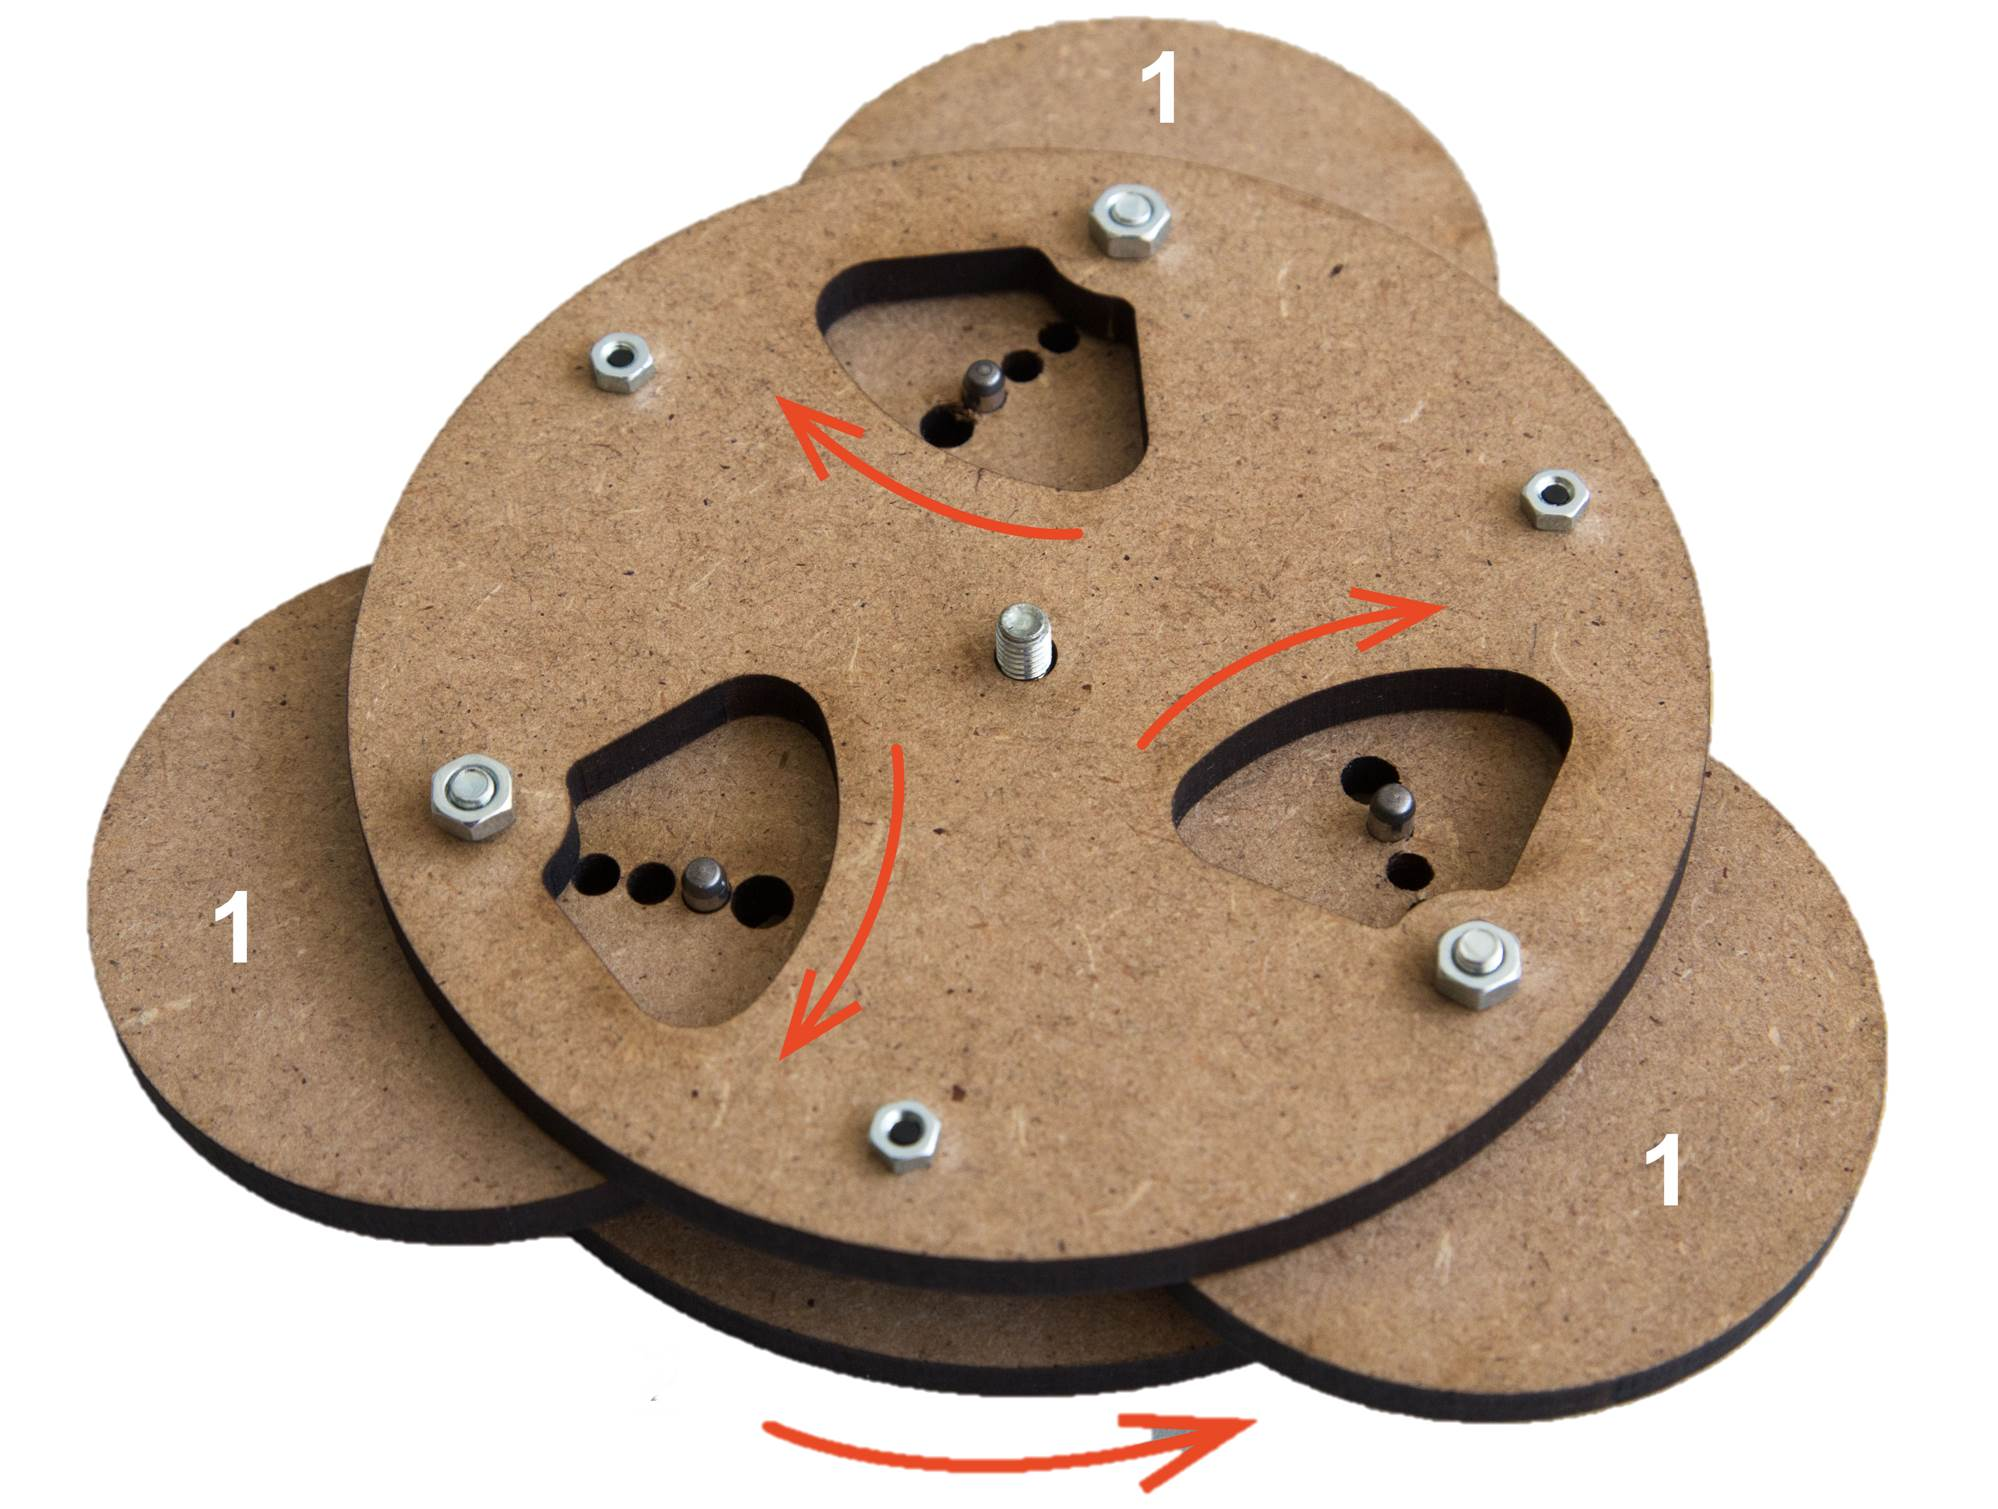
\includegraphics[width=1\textwidth]{Illustrationen/5-Konzept/setzmech_konfig_1.jpg}
	\caption{Teilfunktionsmuster zur Konfiguration des Setzmechanismus}
	\label{fig:setzmech_konfig}
\end{figure}
Folgende Erkenntnisse lieferte das Funktionsmuster:
\begin{itemize}
	\item Die manuelle Verstellung des Radius mittels Kulisse ist möglich. Durch eine Drehbewegung werden die Dornen synchron verstellt.
	
	\item Aus der Geometrie der Kulissen wird erkennbar, dass die maximale Rotation 45° beträgt. Dies muss bei einer allfälligen Evaluation des Antriebs berücksichtigt werden.
	
	\item Am Rand der Kulisse nimmt der Kraftaufwand für eine Verstellung deutlich zu. Es kommt auch vor, dass die Kulisse am Rand kaum in Bewegung gerät. Dies ist damit erklärbar, dass an diesem Punkt die Wirkungslinien der Kulissen normal zueinander stehen und so kein Moment auf die äussere Kulisse wirken kann. Bei einer allfälligen Umsetzung müssen die Wirkungslinien der Kulissen möglichst parallel verlaufen. 
\end{itemize} 
\subsubsection{Topferkennung} \label{sec:Topferkennung_ProveOfConcept}
\textit{(pro)} Als Sensor für die Topferkennung wurde der IR Distanzsensor von Sharp mit der Typenbezeichnung GP2Y0A41SK0F verwendet. Dabei wurde der genannte IR-Sensor mit einem ADC Port des FRDM-Boards verbunden. Es wurde eine Testmessung durchgeführt in der ein Blumentopf mit 14cm Durchmesser vor dem IR-Sensor, mit zwei verschiedenen Geschwindigkeiten, vorbeigeführt wurde. 

\begin{figure}[H]
	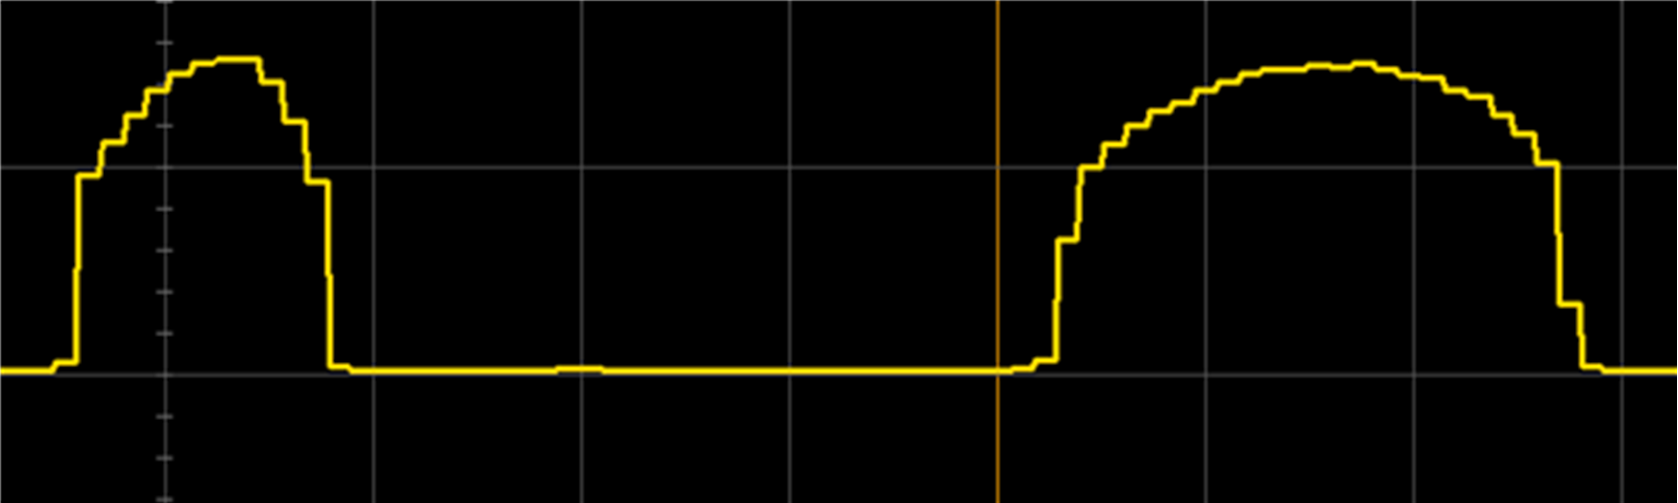
\includegraphics[width=1\textwidth]{Illustrationen/6-Umsetzung/IR_Sensor_Messung.png}
	\caption{Topferkennung, Testmessung}
	\label{fig:IR_Sensor_POC}
\end{figure}

Die Messung wurde mit der Software Segger J-Scope durchgeführt und ist in Abb. \ref{fig:IR_Sensor_POC} illustriert. Die Testmessung ist rein qualitativ und diente als Entscheidungsgrundlage für die Messmethode. Die Messdaten, welche der Sensor liefert, sind nicht linear und zusätzlich invertiert (hoher Pegel = kurze Messdistanz). Um absolute Werte für die Messdistanz zu bekommen, muss das Messsignal gemäss den Angaben im Datenblatt umgerechnet und über eine Lookup-Tabelle aufgelöst werden. Die Form des Topfes ist gut zu erkennen. Aufgrund der gemessenen Daten kann der IR-Sensor für die Topferkennung empfohlen werden.
